\section{Transparency Feature Design}\label{s:design}

This chapter describes the design choices of the mitigation methods in HyperDbg that were made during this project. The designed system of hypervisor transparency is capable of intercepting 3 common detection vectors - CPUID instruction queries, accesses of certain MSR regions and Windows system calls - 
suppressing the ability for any user process or malware to successfully detect that they are running in a virtualized system.

\subsection{General Overview}
The design allows for a modular implementation, where each of the different mitigation handlers are independent of the other ones (see Figure~\ref{fig:feature_diagram}), 
while also being dynamic and allowing the transparency to be toggled on or off at runtime, without requiring a system restart for the guest.
These mitigation features were also designed to be deployable on any system, but the implementation and testing, and thus a guarantee of reliability, 
was performed on a Windows 11 (24H2) bare metal system running on an Intel CPU that supports VT-x hardware virtualization. 

\begin{figure}[tbh]
    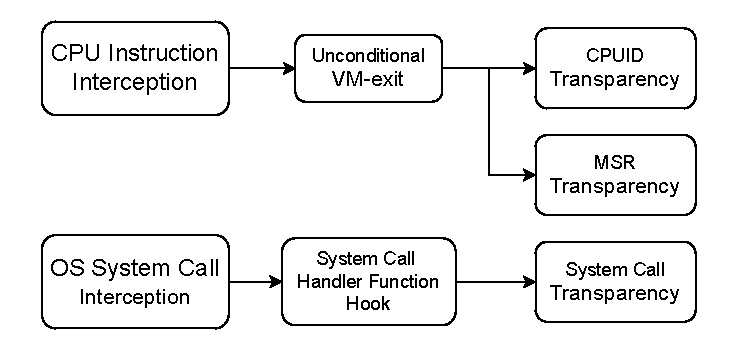
\includegraphics[width=\onecolgrid]{SysDiag1}
    \figcap{Design of the hypervisor detection mitigations}\label{fig:feature_diagram}
\end{figure}

The implementation of these hypervisor transparency features was done based on HyperDbg's 0.13.0 version, on a GitHub fork of the 
project\footnote{The repository of the forked HyperDbg project, where the implementation was done available at: \url{https://github.com/CokeTree3/HyperDbgThesis}}.


\subsection{Feature Design}
\subsubsection{CPUID}
As described by Microsoft\footnote{CPUID instruction description in terms of hypervisor discovery. Microsoft \url{https://learn.microsoft.com/en-us/virtualization/hyper-v-on-windows/tlfs/feature-discovery}}, 
there are two ways the CPUID instruction can be used to check hypervisor presence, reading the “hypervisor present” bit which is at the 31 bit offset of leaf 0x1, that is, the instruction queried with the EAX register set to this value.
\begin{minted}[linenos,frame=single]{nasm}
    MOV EAX, 0x1
    CPUID
\end{minted} 
Or by querying the 0x40000000 leaf for the vendor identifier and max defined leaf range above the 0x40000000 leaf. 
\begin{minted}[linenos,frame=single]{nasm}
    MOV EAX, 0x40000000
    CPUID
\end{minted}
Without mitigations, after calling CPUID with this input value, registers EBX, ECX and EDX will contain the hypervisor vendor string, if it is set as such by the hypervisor.
Both of these methods can be mitigated by intercepting the unconditional VM-exit caused by the CPUID instruction, and changing the return values in the RAX, RBX, RCX and RDX registers. 
By just unsetting the 'hypervisor present bit' in RAX, if the query request in RAX is 0x1, leaving RAX at value 0x4000000, to indicate no higher leaves are defined, and not setting the vendor identifier in the other registers.

\subsubsection{Model Specific Registers}
Similarly, MSR accesses can also be mitigated. Intel defines MSRs in the range 40000000H - 4000FFFFH as reserved~\cite[Volume 4]{Intel-SDM2025} and so they are guaranteed to not be used by hardware. 
Due to this, Microsoft defines them as “Synthetic model specific registers”~\cite{microsoft_hv_interface_reqs}, and consumer hypervisors that conform to the Hyper-V \stress{Hv\#1} interface must define some MSRs in this range. 
In a bare metal system, any access to an undefined MSR causes a general protection error (\stress{\#GP}). In the design, this behavior was emulated, 
so whenever the transparency mode is enabled within HyperDbg, any reads or writes to/from this range will cause a \stress{\#GP} error to be injected to the guest.

\subsubsection{Windows system call interception}\label{syscall_interception}
For the interception and modification of Windows system calls, the approach chosen was to insert an EPT page hook (A feature already implemented in HyperDbg before this thesis\footnote{EPT hooks in HyperDbg. \url{https://docs.hyperdbg.org/commands/extension-commands/epthook}}) 
at the entry point of the Windows system call handler function KiSystemCall64. This function performs the privilege ring swap between user-space and kernel-space. 
Access to the location of this function is obtained from the IA32\_LSTAR MSR. 
This allows HyperDbg to intercept all calls to this function by causing a VM-exit from an EPT violation, and filter the system calls based on their system call number. 
The call number is stored in the RAX register as set up by the user-space system call wrapper functions in the \stress{NTDLL} library~\cite{ntdll-lib}. The general style of these 
wrapper functions is as shown in Listing~\ref{lst:syscall-wrapper}, but with the system call number changed to the appropriate one.
This disassembly also shows that the wrappers move the second argument of the system call, as defined by the x64 fastcall calling convention, 
to R10 from the standard RCX register. This was a detail that was considered during the development.

At the point when the EPT hook is triggered, the system has just transferred the context to kernel space and no execution relating to the requested system call has been done. 
To get to a point in the execution path where data have been written to any memory buffers or the return values have already been set 
requires returning control back to the guest system and intercepting the execution path once more. Preferably, before the control is passed back to the calling user-space process or API function. 
The approach chosen was to set the trap flag in the guest RFLAGS user-space register for the specific thread, which during the interception point is stored on R11, moved there by the SYSCALL instruction~\cite[Volume 2B]{Intel-SDM2025}. 
Once the execution returns to the user-space via the SYSRET instruction, and the user-space RFLAGS are restored, the first instruction will immediately trigger a single-step trap due to the TRAP flag
being set. HyperDbg intercepts this and gives an opportunity to access and modify the return value that the user-space process will be receiving from the system call. 
As many system calls also provide data, more than just a return value, at this point HyperDbg can also read and modify any memory buffers that were 
passed as arguments when the system call was invoked. This callback approach to system call interception allows HyperDbg to filter and only intercept 
the offending system calls (see Table~\ref{tab:syscalls}) and greatly improves performance over intercepting and causing VMX mode changes multiple times on every system call made.

\subsubsection{Modification of system call behavior}
Once the system calls can be intercepted, the chosen non-transparent calls are filtered, and an entry handler for each one can be created. 
These functions execute at the entry point of the system call execution in the kernel, as triggered by the EPT page hook. 
These handlers range from simply setting the trap flag for all calls to the specific system call, to reading user-space buffers written by the caller process, 
filtering the kernel access calls even further. The handler might also corrupt some register values, to trigger an error code to be generated by the kernel 
instead of executing the requested data query. As an example, the Windows system call NtQueryAttributesFile\footnote{NtQueryAttributesFile system call. Microsoft. \url{https://learn.microsoft.com/en-us/windows/win32/devnotes/ntqueryattributesfile}}, 
which retrieves basic information on a specific file or directory, requires 2 arguments: an input structure and a buffer to write the queried information to.
A process attempting to detect a hypervisor might execute this system call on a number of common files that commercial hypervisor vendors might add to a guest system, 
as well as driver files present in the system. The approach taken for mitigating this is to report errors when a query for a known hypervisor specific file is being accessed. 
To achieve this, the system call entry handler has to read the input structure from the user-space virtual pointer, check if the call is a query for these \stress{"bad"} files, 
and only then deploy the mitigations. Which in the case of NtQueryAttributesFile, is to set the trap flag and resume the kernel execution, 
as the actual mitigation has to happen after the kernel returns to user-space.

Once the kernel executes the SYSRET instruction and returns to user-space, the inserted trap flag causes another VM-exit and based on the system call number stored in a list, 
another handler can be called for this callback. At this point in the execution path of system calls, the return value has already been set on RAX and the user-space buffers 
have been written to, if required, by the kernel. This allows the transparent mitigation handlers to read these buffers and modify any data in them 
that could reveal hypervisor presence, such as removing active processes and loaded drivers from their respective lists 
or spoofing the vendor identification in Windows registry key or firmware data.
The mitigations take place in VMX root mode and since these pointers given in the arguments are from the calling processes virtual address space, 
accessing them directly is not possible, so a translation layer needs to be added. The method chosen was to read and copy the data from the translated physical address to a spare memory buffer, 
either on the stack or to an allocated non-paged memory on the heap. From there, modifications of the data in these buffers could be performed, as required based on the system call, 
and then written back to the user-space buffer physical address.
The return values are also spoofed at this point, if needed, by updating the RAX register value. In most cases, by setting the value as an error code instead of the success code of 0x0. 

NtQuerySystemInformation is a system call that can retrieve many types of information on the system, the query is defined by an argument, 
a class value from the \stress{SYSTEM\_INFORMATION\_CLASS} enumeration defined in the NT API~\cite{ntdll-lib}. 
Although not all class data could contain hypervisor revealing data, some of them do. The designed system call interception system mitigates many 
but not all of the query classes. Seen in Table~\ref{tab:QSI-classes}, is a list of the \stress{SYSTEM\_INFORMATION\_CLASS} classes that could be used for hypervisor detection.

\begin{table}[tb]
    \centering
    \tabcap{Some SYSTEM\_INFORMATION\_CLASS classes with a possible use in hypervisor detection}\label{tab:QSI-classes}
    \taburulecolor{black!45}
    \begin{tabu}{l|c|c}
        \toprule
        \multirow{2}{*}{\thead{Name}} &
            \thead{Class} &
            \thead{Implemented} \\
        &
            \thead{number} &
            \thead{in HyperDbg}\\
        \midrule
        SystemProcessInformation
            & 0x05 & \checkmark \\
        SystemModuleInformation
            & 0x0B & \checkmark \\
        SystemKernelDebuggerInformation
            & 0x23 & \checkmark \\
        SystemFirmwareTableInformation
            & 0x4C & \\
        SystemHypervisorInformation
            & 0x5B&\\
        SystemHypervisorDetailInformation
            & 0x9F &\\
        SystemProcessIdInformation
            & 0x58 &\\
        SystemCodeIntegrityInformation
            & 0x67 & \checkmark \\
        SystemHandleInformation
            & 0x10 &\\
        \bottomrule
    \end{tabu}

\end{table}

The values and returned structures were obtained from the NT API documentation provided by the \stress{System Informer} project\footnote{Native API online documentation, based on the System Informer. \url{https://ntdoc.m417z.com/}}.

Multiple hypervisor detection methods commonly used rely on querying for the system firmware and vendor data. On Windows many of these queries are carried out with system calls, 
allowing HyperDbg to intercept them. To appear genuine, when the transparency mode is enabled, a random genuine vendor is chosen from a preset list of numerous genuine computer system and component vendors. 
Any queries for data through system calls that contain hypervisor vendor data, will always report back the same spoofed vendor data, bypassing any hypervisor checks done by the user process.

In the context of Windows, one commonly used approach for obtaining system information is by using the Windows Management Instrumentation (WMI)\footnote{Windows Management Instrumentation documentation. Microsoft. \url{https://learn.microsoft.com/en-us/windows/win32/wmisdk/wmi-start-page}}.
This API provides the user with an interface through which to query and modify many aspects of the operating system. 
Importantly, it can be used in parallel to direct system calls to obtain system information that might reveal the hypervisor~\cite{graeber2015abusing}.
For this thesis, WMI related detection methods did not have mitigations developed as the layout of the WMI structure is relatively spread out and 
does not interact with the kernel through an easily detectable system call, frequently not going through the kernel at all~\cite{wmi-structure}.



%%% Local Variables:
%%% mode: latex
%%% TeX-master: "../thesis"
%%% End:
